% main.tex - 科研项目学习笔记模板
% !TeX root = main.tex
%%%%%%%%%%%%%%%%%%%%%%%%%%%%%% DOCUMENT 
\documentclass[12pt]{report}

%%%%%%%%%%%%%%%%%%%%%%%%%%%%%% PACKAGES

% 中文支持(XeLaTeX 编译)
\usepackage[UTF8]{ctex}
\usepackage{xeCJKfntef} 

% \setCJKmainfont{HanziPen SC}
% \setmainfont{HanziPen SC}


% 页面设置
\usepackage[a4paper, left=20mm, right=20mm, top=15mm, bottom=15mm]{geometry}

\PassOptionsToPackage{dvipsnames,svgnames,x11names}{xcolor}
\usepackage{xcolor}


% 数学环境及符号
\usepackage{amsmath, amssymb, amsfonts, amsthm,amsopn}
\usepackage{tensor}              % 张量指标管理
\usepackage{mathtools}           % amsmath增强
\usepackage{physics}             % 物理公式快捷命令
             % Dirac符号
\usepackage{bbold}               % 数学黑体
\usepackage{dsfont}              % 另一种数字体
\usepackage[mathscr]{eucal}     % 花体字母
\usepackage{tensor}              % 张量指标管理
\usepackage{simpler-wick}       % Wick记号
\usepackage{mathrsfs}            % 另一种花体字母

% 颜色与图形相关
\usepackage{graphicx}           % 插图支持
\usepackage{float}              % 浮动体控制
\usepackage{tikz}               % 绘图库
\usetikzlibrary{math}           % tikz数学扩展
\usepackage{geometry}
% 表格与列表
\usepackage{makecell}           % 表格多行换行
\usepackage{multicol}           % 多栏排版
\usepackage{colortbl}           % 表格颜色
\usepackage{enumitem}           % 列表自定义

% 其他辅助
\usepackage{framed}             % 有边框环境
\usepackage{tcolorbox}          % 灵活盒子环境
\tcbuselibrary{breakable}       % 盒子内容分页
\usepackage{thmtools}           % 定理环境管理
\usepackage{thm-restate}        % 定理重述
\usepackage{showlabels}         % 显示标签,调试用(完成后可注释)
\usepackage[normalem]{ulem}     % 下划线、删除线
\usepackage{hyperref}           % 超链接(最后加载)
\usepackage{cleveref}           % 智能引用(紧跟hyperref)
\usepackage{soul}

% 自定义宏包
\usepackage{macros}

% 一个中文可以高亮的包
\usepackage{cjkhl}
\definecolor{lightblue}{rgb}{.8,.8,1}

%%%%%%%%%%%%%%%%%%%%%%%%%%%%%% 自定义命令
\newcommand{\tml}{Teichmüller space}
\newcommand{\hil}{Hilbert space}
\newcommand{\mtc}{Modular Tensor Category}

%%%%%%%%%%%%%%%%%%%%%%%%%%%%%% BEGINNING OF THE DOCUMENT

\begin{document}

\title{\boldmath Liuy的latex科研及学习笔记模板}
\author{X. D. H.}

\maketitle

\begin{abstract}
  这个是我的Latex科研学习模板!我是用这个模板完成科研工作的记录,学习内容的记录。我会比较系统性的整理知识,同时也是用了很多的快捷方法。 
\end{abstract}

\tableofcontents

\chapter{科研主体内容}
这里我们阶段性记录科研取得的结果或者一些中间思考得到的结果。其中也有内容启发我们下面一步做什么。这里主要集中放置科研结果。


\chapter{知识补充!}
这里记录一些补充的知识!!!

\section{框框}\label{sec:框框} % (fold)

记录知识之中我们会经常使用到一些框框我设置为一些macros可以使用。

\imp{重要的内容也是最常用的}{
  这里是重要的内容!!特别的重要
}
\tip{一些点}{
  这里是一些没有最重要但是需要提出来的点
}
\ques{问题}{
  这里记录我遇到的问题
}
\rmk{这个也是常用记录一些特殊的remark!!}
这几个是最重要的内容
% section 框框 (end)

\section{特殊使用}\label{sec:special} % (fold)
学习显然并不是一次就能学懂我会用


\YL{这个来进行一些个人的评论以及一些疑问的地方!!}
% section 特殊使用 (end)



\chapter{chap1 小呆花}\label{chap:chap1} % (fold)
我们根据学习的内容进行自行分类进行学习。我加油!

下面我们可以学习时候使用一些图片,图片在assert的文件夹之中比如下面这个。

\begin{figure}[H]
  \centering
  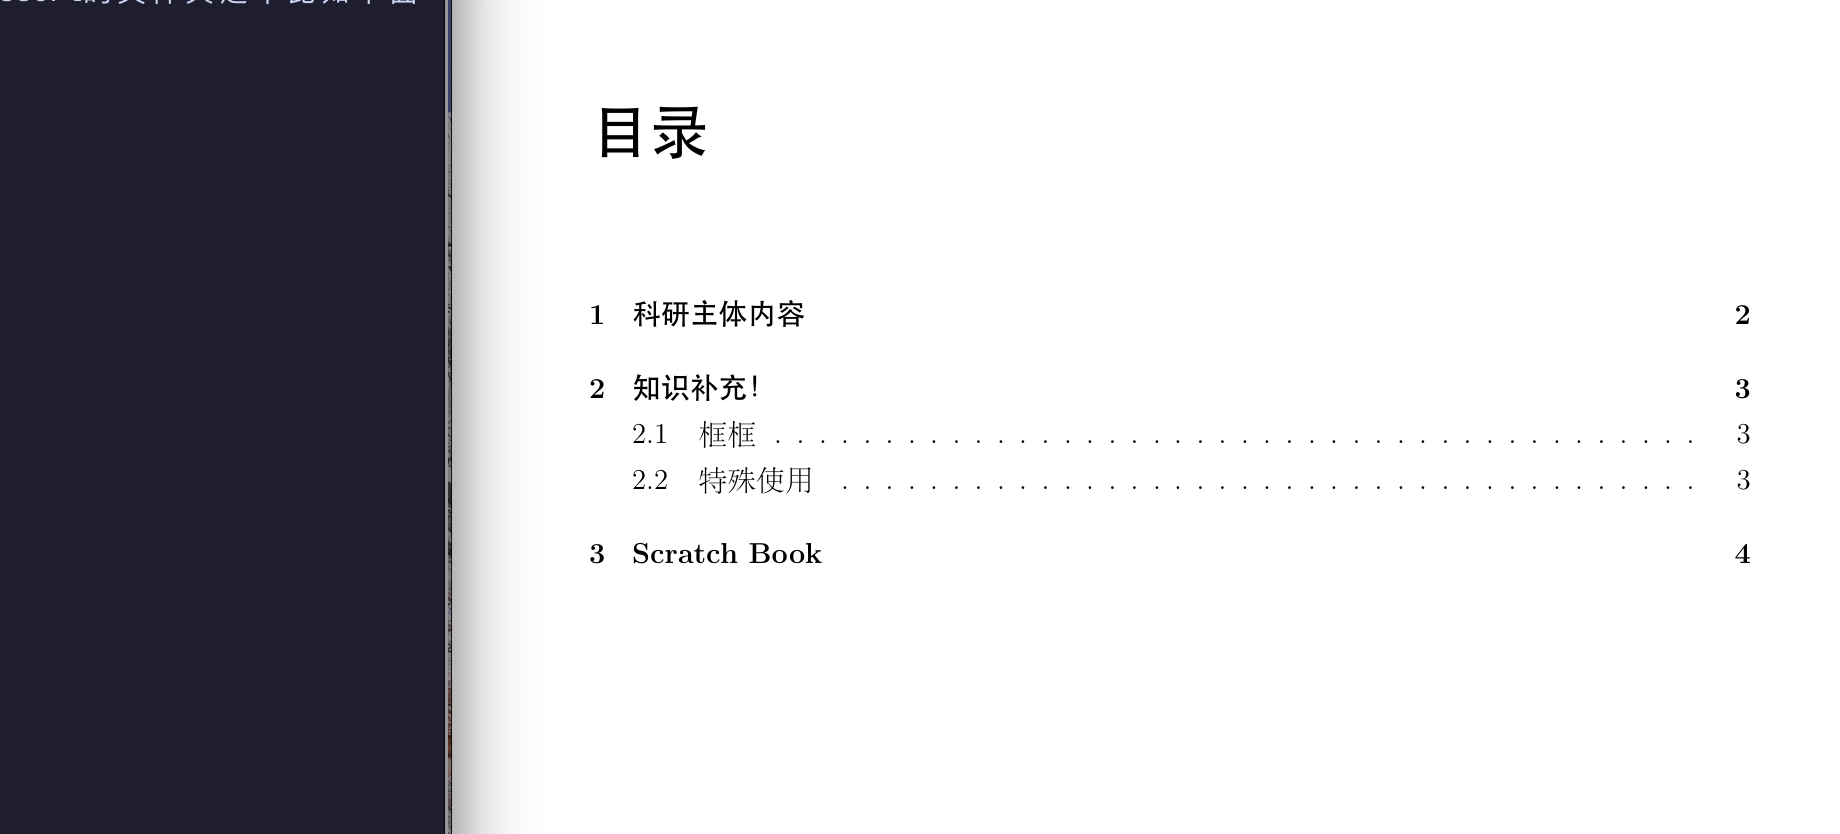
\includegraphics[width=0.75\textwidth]{assets/testfile.png}
  \caption{this is a test file}
  \label{fig:testfile}
\end{figure}

% chapter chap1 小呆花 (end)

\chapter{Scratch Book}
\sout{这里会放一些写的很混沌,但懒得扔掉的东西呜呜呜呜!!!}


\end{document}
